La disciplina è nata dall'esigenza di gestire l'enorme quantità di dati disponibili, in particolare nel contesto delle biblioteche, delle raccolte di documenti e,
più recentemente, del mondo digitale e dell'Internet.

Negli Anni '60 e '70 si è vista la crescita delle prime basi di dati elettroniche e dei primi sistemi di IR automatizzati. Il progetto MEDLARS presso la National Library of Medicine negli Stati Uniti è stato uno dei primi esempi di successo nell'applicazione dell'IR alle pubblicazioni mediche. Nel 1965, Gerard Salton ha sviluppato il modello matematico di "Term Frequency-Inverse Document Frequency" (TF-IDF), che è ancora oggi una tecnica chiave nell'IR.

Negli Anni '80 e '90 l'avvento dei computer personali e il boom delle reti informatiche hanno reso possibile l'accesso alle informazioni da remoto. Motori di ricerca come Archie, Gopher e, più tardi, il famoso WebCrawler, hanno iniziato a indicizzare e cercare pagine Web.

Gli Anni 2000 hanno visto la nascita dei motori di ricerca moderni, tra cui Google che ha introdotto algoritmi di ranking più avanzati basati su link e testo. Il concetto di "PageRank" è stato cruciale per migliorare la qualità dei risultati di ricerca.

Negli Anni 2010 l'IR è diventato sempre più legato all'apprendimento automatico e all'intelligenza artificiale. I motori di ricerca hanno iniziato a utilizzare algoritmi di apprendimento per personalizzare i risultati in base al comportamento dell'utente.

Oggi l'IR è diventato una parte fondamentale della nostra vita quotidiana. Motori di ricerca, sistemi di raccomandazione e algoritmi di classificazione guidano il nostro accesso all'informazione. Con l'avvento del Web semantico e dell'elaborazione del linguaggio naturale, l'IR sta evolvendo per comprendere il significato contestuale delle query e dei documenti, portando a risultati di ricerca ancora più raffinati.

In sintesi, la storia dell'Information Retrieval è una progressione che va dall'organizzazione manuale delle informazioni alla creazione di potenti motori di ricerca guidati dall'intelligenza artificiale. Questo campo in continua evoluzione gioca un ruolo cruciale nell'aiutare le persone a trovare e comprendere le informazioni nel mare sempre crescente di dati digitali.

\begin{figure}
    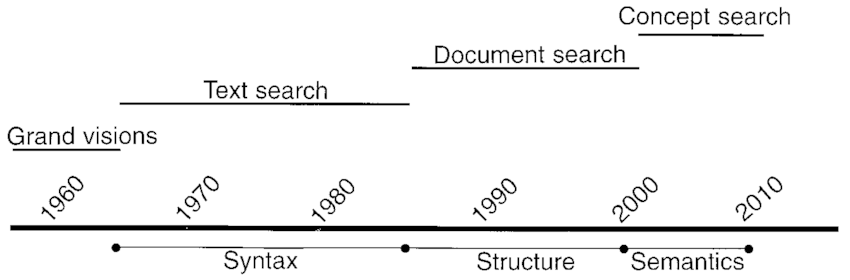
\includegraphics[width=0.75\pdfpagewidth]{images/timelineir.png}
    \caption{Timeline dell'Information Retrieval}
\end{figure}